\section{Performantie}
\label{sec:evaluatie-performantie}

%%%%%%%%%%%%

Op figuur \ref{fig:performantie} wordt de gemiddelde downloadtijd van de POC en login, zowel niet gecachet als gecachet, voor de vier raamwerken getoond.

\begin{figure}[H]
  \centering
  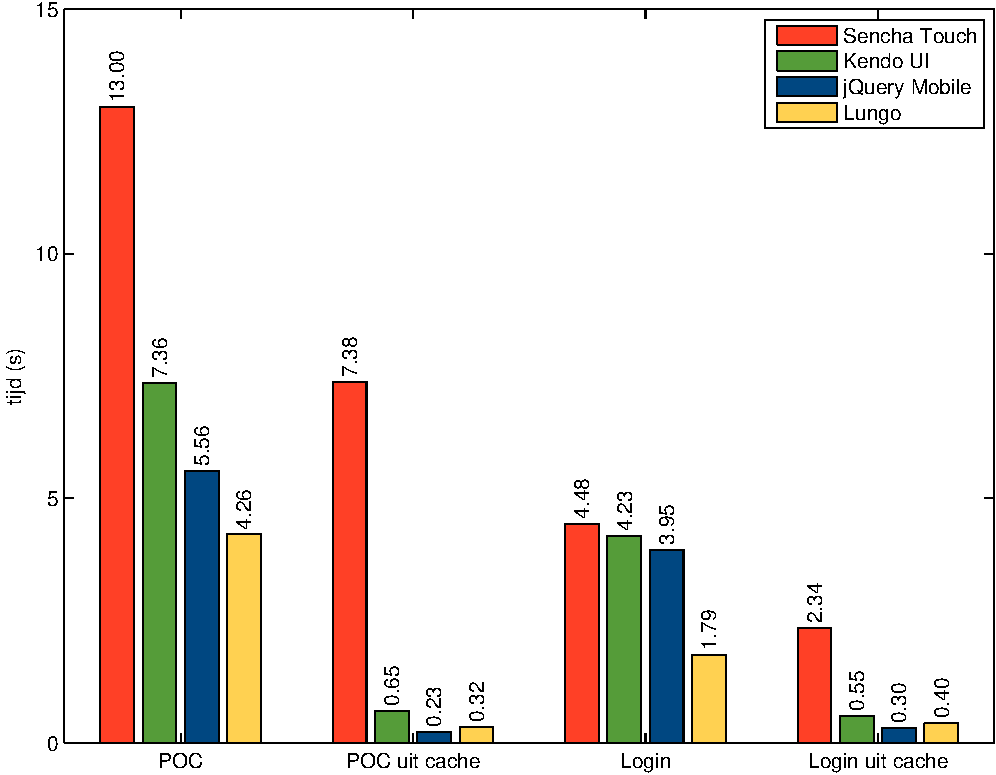
\includegraphics[width=\textwidth]{figuren/performance.pdf}
  \caption{Gemiddelde downloadtijd van POC,  POC uit cache,  login en login uit cache voor elk raamwerk (minder is beter).}
  \label{fig:performantie}
\end{figure}

\lungo{} behaalt de eerste plaats.
Als er gekeken wordt naar de POC heeft \lungo{} maar een derde van de tijd nodig ten opzichte van het traagste raamwerk, \st.
\jqm{} en \kendo{} behalen respectievelijk een tweede en derde plaats.
Aangezien niet alles werd geïmplementeerd in de POC voor \lungo{}, zou men kunnen stellen dat dat de reden is.
Als er echter wordt gekeken naar de loginapplicatie waar alles wel vergelijkbaar is, dan blijft \lungo{} het snelste raamwerk.
Het is zelfs meer dan de helft sneller dan \jqm{}, \kendo{} of \st{}.
Deze drie raamwerken behalen quasi dezelfde opstarttijd, maar ook hier is \st{} terug de traagste.

Als naar de gecachte versie wordt gekeken voor zowel POC als loginapplicatie, scoren \kendo{}, \jqm{} en \lungo{} hetzelfde.
Daarentegen behaalt \st{} telkens een vele tragere tijd.
Enerzijds komt dit doordat de drie eerstgenoemde raamwerken enkel gebruik maken van HTML5 Application Cache.
\st{} gebruikt daarnaast ook nog een eigen mechanisme (zie \ref{sec:performantie-st}) waardoor de grotere laadtijd wordt verklaard.
Anderzijds gebruiken de drie eerstgenoemde raamwerken Yeoman om de applicatie te bouwen.
De webapplicaties gemaakt \st{} gebruiken daarentegen Sencha Cmd.

%%%% De cache factor van ST is constant (gemiddeld 1,8)
%%%% De andere raamwerken hebben een beduidend grotere cache factor 

Indien \st{} buiten beschouwen wordt geladen, duurt het eerste keer laden van de POC gemiddeld 5,73 seconden. 
Het laden van de gecachete versie duurt slechts gemiddeld 400 milliseconden.
De eerste keer laden van de loginapplicatie duurt gemiddeld 3,32 seconden.
Indien deze werd gecachet, duurt dit nog slechts gemiddeld 420 milliseconden.
Dit zijn aanvaardbare tijden volgens Jakob Nielsen~\cite{Nielsen1993}.
Hij stelt dat indien de tijden onder 1 seconde blijven, de gebruiker de vertraging waarneemt, maar het zijn gedachtengang niet belet.
Tussen de 1 en 10 seconden dient er feedback over het laden te worden gegeven aan de gebruiker.
De browser neemt hiervoor de taak op zich door bij het laden een indicator te tonen.

%TODO: moet Jakob niet worden verplaatst naar het vergelijkingshoofdstuk? 

%%%%% BEGIN HIER HIERSCHRIJVEN %%%%%%

%TODO uitleggen dat we de JS perfomrantie hebben proberen op te meten
% het is gelukt voor jQM en Kendo, maar niet voor ST en Lungo
% eventueel referenties naar vragen op so
% daarom werd besloten om deze meting er uit te laten ,aangezien we maar toch 2 frameworks konden meten
% dit wordt vervangen door een subjectieve lijsttest (+ fout tegen nielson, tijdsbudget, we moesten 5 gebruikers gebruikers hebben, maar hadden er maar 2, met name de auteurs zelf)
% hierdoor wordt de formule aangepast, aangezien lijsttest (uitgedrukt in eenheid) en downloadtijd (uitgebrukt in seconden) niet kunnen worden opgeteld, daarom als fator gebruiken
% van de totale downloaded wordt gedeeld met die factor 

% table subjectieve testen loginlijsten toeveogen (8 devices)

% VERWERKEN TEKST SANDER
%Een andere test om de score te toetsen kijkt naar de gebruikservaring.
%Hiervoor zal de lijst van $850$ elementen worden gebruikt die getoond wordt na aanmelden op de loginapplicatie.
%De auteurs zullen de ervaring bij het scrollen van de lijst vergelijken op de acht apparaten.
%De ervaringen per apparaat zullen vervolgens relatief ten opzichte van elkaar beoordeeld worden.

% onderstaande sectie hierwerken, gebruikservaring is geen verklaring meer.
%\paragraph{Gebruikservaring}
Een andere test om de score te toetsen kijkt naar de gebruikservaring.
Hiervoor werd door de lijst van $850$ elementen gescrold, die getoond wordt na aanmelden op de loginapplicatie.
De test werd uitgevoerd op de acht apparaten van tabel~\ref{tabel:toestellen-hci}.
De totaalscores voor alle devices is in tabel~\ref{tabel:performantie-verklaring} terug te vinden.
\st{} behaalde de maximale score.
Dit wil zeggen dat op alle toestellen het scollen door de lijst van \st{} het vlotst ging.
\jqm{} werd zes keer als tweede beste beoordeeld. 
Op de \htc{} liep \kendo{} vlotter,  op de \ipadi{} was \lungo{} nummer twee.
De lijst genereren met \kendo{} op iOS toestellen was onmogelijk omdat de applicatie de browser liet crashen.
Op Android toestellen kon de \kendo{} lijst echter wel worden getoond.
%TODO: dat weten we niet, enkel dat het crasht.
% we hebben zowel de reden niet verder gecontroleerd alsook de grens tot waar het niet crasht wegens tijdsbudget
Dit wil zeggen dat de overhead die \kendo{} genereerd, het maximale toegelaten geheugen van het iOS besturingssysteem overschrijdt.
De score van \kendo{} is dus slechts voor vier apparaten.

% nieuwe formule
% nieuwe tabel: 3 rijen (totale download, factor, nieuw abs totaal)

%%%%% TOT HIER HIERSCHRIJVEN %%%%%%

In wat volgt zullen metrieken worden besproken die de score van de performantie zullen duiden.
De data van de metrieken is weergegeven in tabel~\ref{tabel:performantie-verklaring}.

\paragraph{Google Page Speed}
De score op 100 die Google Page Speed~\cite{Morgan2011} aan de applicatie toekent kan in tabel~\ref{tabel:performantie-verklaring} worden teruggevonden voor zowel de POC als de loginapplicatie.
\st{} scoort het best ($96$),  gevolgd door \lungo{} ($88$),  \jqm{}($71$) en \kendo{}($66$).
Dezelfde trend kan bij de loginapplicatie teruggevonden worden.
Het enige verschil is dat bij de POC van \kendo{} de afbeeldingen niet optimaal gecomprimeerd zijn.
Bij de loginapplicatie van \kendo{} is dit wel gebeurd.
Door deze uitbreiding krijgt de loginapplicatie van \kendo{} en beter score dan \jqm{}.

Er kan geconcludeerd worden dat Sencha Cmd de applicatie optimaal weet te bouwen.
Hoewel \st{} de meeste tijd vraagt om te laden, zal het na het laden sneller werken.
Dit wordt bevestigd in de test over gebruikservaring.

\paragraph{Downloadgrootte en HTML-code}
De HAR-bestanden die werden gebruikt om de laadtijd op te meten bevatten ook de grootte van de pakketten die moeten worden opgehaald.
Omdat pakketten verloren gaan zullen ontvangen bestanden incompleet zijn en moeten ze worden herverzonden. %TODO Sander: klopt dat?
Hierdoor zal het aantal ontvangen bytes variëren van meting tot meting.
De performantietesten werden op acht toestellen uitgevoerd en elke test werd drie keer uitgevoerd.
Het gemiddelde van alle downloadgroottes bepaalt de grootte zoals deze kan worden teruggevonden in tabel~\ref{tabel:performantie-verklaring}.
Bij de POC moet \st{} de meeste data ophalen ($1126.4$kB),  gevolgd door \kendo{} ($194.65kB$kB), \lungo{} ($249.08$kB) en \jqm{} ($194.65$kB).
Opmerkelijk is dat \lungo{} meer data moet ophalen maar toch een snellere laadtijd behaald.
Ook het verschil in downloadgrootte tussen de POC en loginapplicatie is opmerkelijk.
Bij \jqm{} kan slechts een daling van $4.74\%$ worden waargenomen.
\st{} en \lungo{} waren gelijkaardig en de downloadgrootte daalde respectievelijk met $78.02\%$ en $76.01\%$.
De reductie in data bij \kendo{} was $45.30\%$.

Bij alle applicaties werd de \js{}- en CSS-code verkleind en samengevoegd.
De HTML-code werd niet gewijzigd.
Tabel~\ref{tabel:performantie-verklaring} bevat het aantal lijnen HTML-code dat moest worden opgehaald.
Hieruit is duidelijk te zien welke raamwerken opmaakgedreven zijn.
%TODO Sander: moet hier nog meer vermeld worden?

\begin{table}[H]
\centering
\pgfplotstabletypeset[
  begin table=\begin{tabular}{p{8cm} p{1cm} p{1cm} p{1cm} p{1cm}},
  end table=\end{tabular},
  skip coltypes=true,
  col sep=comma,
  string type,
  header=true,
  columns={Performantie Metrieken,jQM,ST,Kendo,Lungo},
  columns/Performantie/.style={column name=\textbf{Performantie Metrieken}, column type={l}},  
  columns/ST/.style={column name=\textbf{\sta}, column type={c}},
  columns/jQM/.style={column name=\textbf{\jqma}, column type={c}},
  columns/Kendo/.style={column name=\textbf{\kendoa}, column type={c}},
  columns/Lungo/.style={column name=\textbf{\lungoa}, column type={c}},
  every head row/.style={
    before row=\toprule,
    after row=\midrule},
  every last row/.style={
  	before row=\midrule,
    after row=\bottomrule}
]{tabellen/performantie/performantie-verklaring.csv}
\caption{Metrieken gebruikt bij de verklaring van performantiecriterium voor \st{}~(\sta), \kendo{}~(\kendoa), \jqm{}~(\jqma) en \lungo{}~(\lungoa).}
\label{tabel:performantie-verklaring}
\end{table}


\subsection{\st}
\label{sec:performantie-st}
Op figuur~\ref{fig:performantie-st} worden de gemiddelde downloadtijd van \st{} getoond op elk apparaat.

Voor de POC is een dalende downloadtijd waarneembaar wanneer het Android-apparaat recenter wordt.
De downloadtijd van de POC op de \gs{} duurde gemiddeld $31.43$s!
Gemiddeld moeten Android toestellen $5$ seconden langer laden in vergelijking met iOS toestellen.
Dit gemiddelde wordt sterk beinvloed door de trage laadtijd van de \gs{}.

\st{} heeft een andere aanpak voor het cachen van een applicatie door de introductie van een \term{Delta-update} mechanisme.
Dit mechanisme wil voorkomen dat bij een kleine aanpassing in de code,  alle bestanden opnieuw moeten worden opgehaald die in het \term{manifest} bestand staan opgelijst.
De \term{Micro-loader} is verantwoordelijk voor het asynchroon ophalen van all benodigde \js{}- en CSS-bestanden.
Na het bouwen van een applicatie met Sencha Cmd,  zullen de gewijzigde bestanden gearchiveerd worden en worden de veranderingen tussen elke versie opgeslagen.
Na het laden van de applicatie, zal de \code{Micro-loader} met een GET-verzoek controleren op wijzigingen.
Dit GET-verzoek zal de grootste tijd voor zijn rekening nemen bij de laadtijden bij applicaties uit de cache.
\st{} heeft er dus voor gekozen om aan performantie in te boeten ten voordele van het update mechanisme.
%TODO referentie http://www.sencha.com/blog/behind-sencha-command-and-the-build-process


Een laatste opmerking die bij \st{} moet worden gemaakt, is dat AJAX-verzoeken van een \code{proxy} naar een ander domein altijd vooraf worden gegaan met een OPTIONS-verzoek.
Dit is een verzoek om informatie over de beschikbare opties van het communicatiekanaal op te vragen.
Standaard zet \st{} de \code{X-Requested-With} op XMLHttpRequest en hierdoor zal de browser een OPTIONS-verzoek als \term{preflight} sturen.
%Setting custom headers on XHR requests triggers a preflight request. %http://remysharp.com/2011/04/21/getting-cors-working/
%http://stackoverflow.com/questions/10236056/when-loading-a-store-in-sencha-touch-2-how-can-i-stop-the-additional-options-ht
% POST /resources/userService/login?_dc=1368367749599 HTTP/1.1
% Host: kulcapexpenseapp.appspot.com
% Connection: keep-alive
% Content-Length: 54
% Origin: http://sandervanloock.github.io
% User-Agent: Mozilla/5.0 (X11; Linux i686) AppleWebKit/537.11 (KHTML, like Gecko) Chrome/23.0.1271.64 Safari/537.11
% Content-Type: application/x-www-form-urlencoded; charset=UTF-8
% Accept: */*
% Referer: http://sandervanloock.github.io/HTMobieL/Sencha/build/ExpenseApp/production/index.html
% Accept-Encoding: gzip,deflate,sdch
% Accept-Language: nl-NL,nl;q=0.8,en-US;q=0.6,en;q=0.4
% Accept-Charset: ISO-8859-1,utf-8;q=0.7,*;q=0.3
% 
% Accept:*/*
% Accept-Charset:ISO-8859-1,utf-8;q=0.7,*;q=0.3
% Accept-Encoding:gzip,deflate,sdch
% Accept-Language:nl-NL,nl;q=0.8,en-US;q=0.6,en;q=0.4
% Connection:keep-alive
% Content-Length:23
% Content-Type:application/x-www-form-urlencoded; charset=UTF-8
% Host:kulcapexpenseapp.appspot.com
% Origin:http://sandervanloock.github.io
% Referer:http://sandervanloock.github.io/HTMobieL/Sencha/build/ExpenseApp/production/index.html
% User-Agent:Mozilla/5.0 (X11; Linux i686) AppleWebKit/537.11 (KHTML, like Gecko) Chrome/23.0.1271.64 Safari/537.11
% X-Requested-With:XMLHttpRequest

\begin{figure}[H]
  \centering
  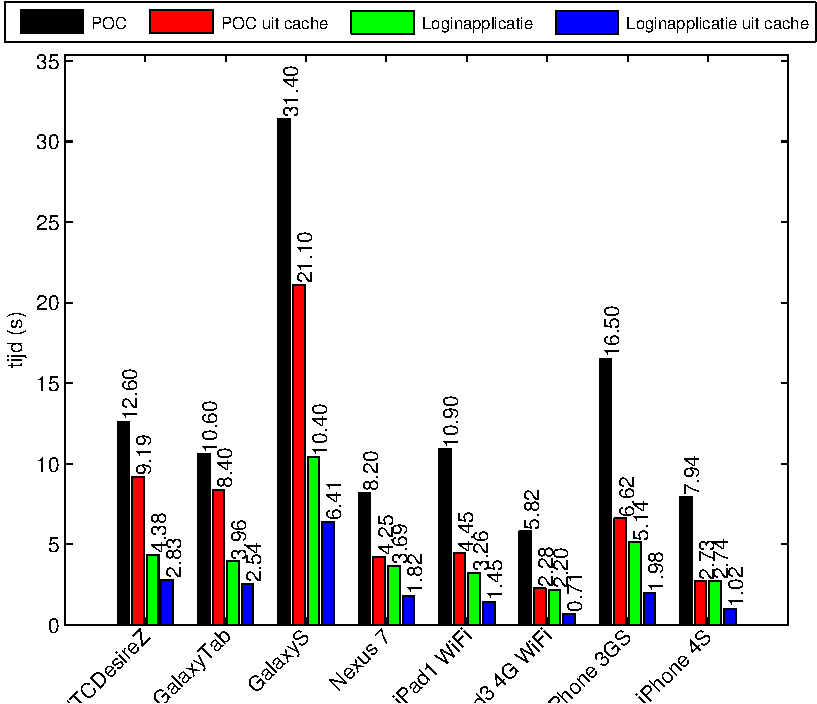
\includegraphics[width=\textwidth]{figuren/performance-st.pdf}
  \caption{Gemiddelde downloadtijden van \st{} voor POC,  POC uit cache,  Login en Login uit cache voor elk apparaat.}
  \label{fig:performantie-st}
\end{figure}

\subsection{\kendo}
Op figuur~\ref{fig:performantie-kendo} worden de gemiddelde downloadtijd van \kendo{} getoond op elk apparaat.

De \gtab{} vertoond de hoogste laadtijd,  gevolgd door de \iphoneiii{} en \htc.
Opmerkelijk is dat de gecachete versie van de loginapplicatie op de \nexus{} $10$ keer trager laadt dan de gecachete versie van de POC.
Het ophalen van een gecachete applicatie werkt bij de \gs{} het traagst.

Bij \kendo{} is er geen opmerkelijk verschil waarneembaar tussen Android en iOS toestellen (Android gemiddeld slechts $60$ms trager).

\begin{figure}[H]
  \centering
  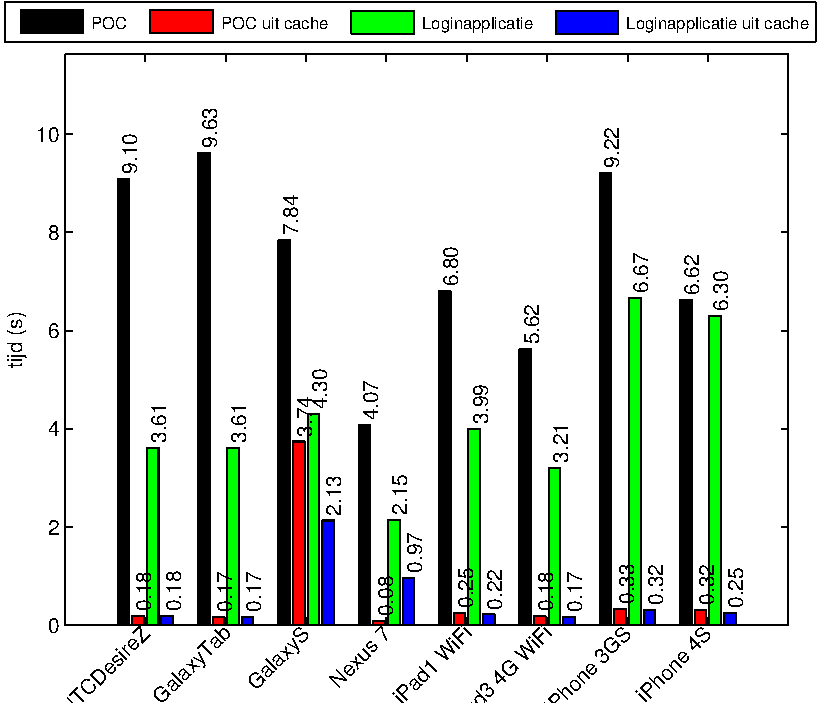
\includegraphics[width=\textwidth]{figuren/performance-kendo.pdf}
  \caption{Gemiddelde downloadtijden van \kendo{} voor POC,  POC uit cache,  login en login uit cache voor elk apparaat.}
  \label{fig:performantie-kendo}
\end{figure}

\subsection{\jqm}
Op figuur~\ref{fig:performantie-jqm} worden de gemiddelde downloadtijd van \jqm{} getoond op elk apparaat.

%TODO Sander: fout (\gs is minst recent...
Voor de POC is een dalende downloadtijd waarneembaar wanneer het Android-apparaat recenter wordt.
Dit is echter ook zo voor de iPads van Apple, maar voor de iPhones stijgt de downloadtijd.
Er zijn minimale verschillen bij de gecachete versie van de POC, waarbij het het langste duurt op de \ipadi{}.

Als de loginapplicatie wordt bekeken, wordt hetzelfde waargenomen als voor de POC.
Enkel bij de Android-apparaten wordt de downloadtijd trager, naarmate het toestel recenter wordt.
Dit is in tegenstelling tot de POC.

Een opmerkelijke waarneming is dat het langer duurt om de gecachete versie van het loginscherm te laden dan de volledige POC.

\begin{figure}[H]
  \centering
  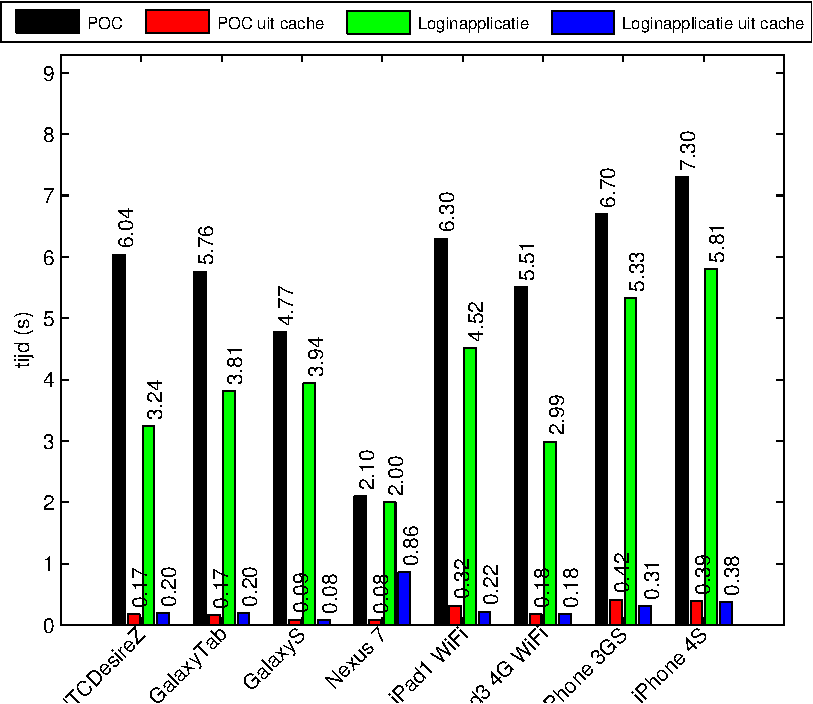
\includegraphics[width=\textwidth]{figuren/performance-jquery.pdf}
  \caption{Gemiddelde downloadtijd van \jqm{} voor POC,  POC uit cache, login en login uit cache voor elk apparaat.}
  \label{fig:performantie-jqm}
\end{figure}

\subsection{\lungo}

\begin{figure}[H]
  \centering
  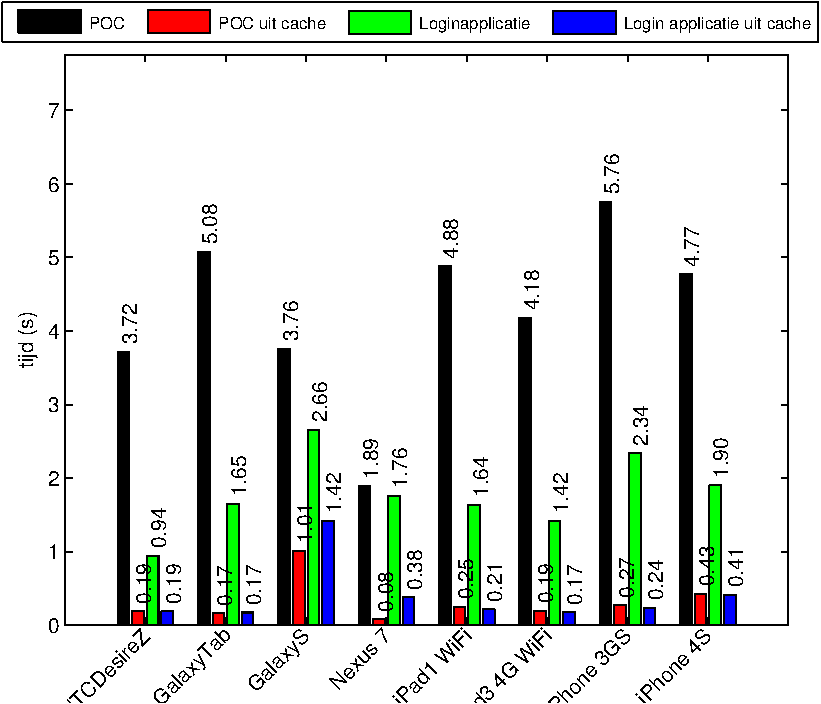
\includegraphics[width=\textwidth]{figuren/performance-lungo.pdf}
  \caption{Gemiddelde downloadtijd van \lungo{} voor POC,  POC uit cache,  Login en Login uit cache voor elk apparaat.}
  \label{fig:performantie-lungo}
\end{figure}
